%%%%%%%%%%%%%%%%%%%%%%%%%%%%%%%%%%%%%%%%%%%%%%%%%%%%%%%%%%%%%%%%%%%%%%
% LaTeX Template: Project Titlepage
%
% Source: http://www.howtotex.com
% Date: April 2011
% 
% This is a title page template which be used for articles & reports.
% 
% Feel free to distribute this example, but please keep the referral
% to howtotex.com
% 
%%%%%%%%%%%%%%%%%%%%%%%%%%%%%%%%%%%%%%%%%%%%%%%%%%%%%%%%%%%%%%%%%%%%%%
% How to use writeLaTeX: 
%s
% You edit the source code here on the left, and the preview on the
% right shows you the result within a few seconds.
%
% Bookmark this page and share the URL with your co-authors. They can
% edit at the same time!
%
% You can upload figures, bibliographies, custom classes and
% styles using the files menu.
%
% If you're new to LaTeX, the wikibook is a great place to start:
% http://en.wikibooks.org/wiki/LaTeX
%
%%%%%%%%%%%%%%%%%%%%%%%%%%%%%%%%%%%%%%%%%%%%%%%%%%%%%%%%%%%%%%%%%%%%%%
%
% --------------------------------------------------------------------
% Preamble
% --------------------------------------------------------------------
\documentclass[paper=a4, fontsize=10pt]{scrartcl}	% KOMA
\usepackage[bottom=1.1in, top=0.9in]{geometry}
\usepackage{lmodern}

\newcommand{\specialcell}[2][c]{%
	\begin{tabular}[#1]{@{}c@{}}#2\end{tabular}}
\usepackage{todonotes}
\usepackage{listings}
\usepackage{graphbox}
\usepackage{hyperref}
\usepackage{twoopt}
\usepackage{adjustbox}
\usepackage[english]{babel}
\usepackage{graphicx}
\usepackage{subcaption}
\usepackage{mwe}
\usepackage{color, colortbl}
\usepackage[protrusion=true,expansion=true]{microtype}	
\usepackage{amsmath,amsfonts,amsthm,amssymb}
\usepackage{tabularx}
\usepackage{float}
\usepackage{tikz} 
\usepackage{xcolor}
\usepackage{listings}
\usepackage{arydshln}
\usepackage{bytefield}


\definecolor{mGreen}{rgb}{0,0.6,0}
\definecolor{mGray}{rgb}{0.5,0.5,0.5}
\definecolor{mPurple}{rgb}{0.58,0,0.82}
\definecolor{backgroundColour}{rgb}{0.95,0.95,0.92}

\newcommand\setrow[1]{\gdef\rowmac{#1}#1\ignorespaces}
\newcommand\clearrow{\global\let\rowmac\relax}
\usepackage{graphicx}
\usepackage[T1]{fontenc}
\definecolor{Red}{rgb}{1,0.7,0.7}
\definecolor{Yellow}{HTML}{FAFAD2}
\definecolor{Green}{HTML}{9ACD32}
\definecolor{Blue}{rgb}{0.5,0.8,1}
\lstset{
	frame=single,
	xleftmargin=15pt,
	xrightmargin=15pt,
	basicstyle=\ttfamily\small
}
\lstdefinestyle{CStyle}{
    backgroundcolor=\color{backgroundColour},   
    commentstyle=\color{mGreen},
    keywordstyle=\color{magenta},
    numberstyle=\tiny\color{mGray},
    stringstyle=\color{mPurple},
    basicstyle=\footnotesize,
    breakatwhitespace=false,         
    breaklines=false,                 
    captionpos=b,                    
    keepspaces=true,                 
    numbers=left,                    
    numbersep=5pt,                  
    showspaces=false,                
    showstringspaces=false,
    showtabs=false,                  
    tabsize=2,
    language=C
}
% --------------------------------------------------------------------
% Definitions (do not change this)
% --------------------------------------------------------------------
\newcommand{\HRule}[1]{\rule{\linewidth}{#1}} 	% Horizontal rule
\newcommandtwoopt*{\myref}[3][][]{%
	\hyperref[{#3}]{%
		\ifx\\#1\\%
		\else
		#1~%
		\fi
		\ref*{#3}%
		\ifx\\#2\\%
		\else
		\,#2%
		\fi
	}%
}

\makeatletter							% Title
\def\printtitle{%						
	{\centering \@title\par}}
\makeatother									

\makeatletter							% Author
\def\printauthor{%					
	{\centering \large \@author}}				
\makeatother							

% --------------------------------------------------------------------
% Metadata (Change this)
% --------------------------------------------------------------------
\title{	\normalsize \textsc{Politecnico di Torino\\GPU Programming} 	% Subtitle
	\\[2.0cm]								% 2cm spacing
	\HRule{0.5pt} \\						% Upper rule
	\LARGE \textbf{\uppercase{Report: PROJECT\\Webcam streaming \& filters}}	% Title
	\HRule{2pt} \\ [0.5cm]		% Lower rule + 0.5cm spacing
	\normalsize 
	\today % Todays date
}

\author{
	Matteo Battilana, Salvatore Gabriele La Greca, Giovanni Pollo
}

\begin{document}
	% ------------------------------------------------------------------------------
	% Maketitle
	% ------------------------------------------------------------------------------
	\thispagestyle{empty}		% Remove page numbering on this page
	
	\printtitle					% Print the title data as defined above
	\vfill
	\printauthor				% Print the author data as defined above
	\newpage
	% ------------------------------------------------------------------------------
	% Begin document
	% ------------------------------------------------------------------------------
	\setcounter{page}{1}		% Set page numbering to begin on this page
	\section{Introduction}

	A classical video streaming algorithm over internet or over any other communication channel is based on the concept of sending not frame by frame as they are but instead they are based on sending the first frame and then the difference between the new one and the previous, where difference here is to be indended pixel-by-pixel difference.\\
	
	If this can be arguable for video with a lower resolution, the heaviness of sending each frame as it is for high video resolution is notable. Let's take as an example a FULL HD video, means that each frame is composed of 1920x1080 pixels where 1920 is the width of the frame while 1080 is the height. Supposing the frame is in RGB24 format, means that each pixel is rapresented by 3 byte (one for each channel R, G, and B).\\
	
	By doing a rapid computation, each frame measures $3 \cdot 1920 \cdot 1080 B = 6220800 B = 5.93 MB $. Supposing now the video used by example is a 30 fps video, means that each second we have 30 frame, each of one measures 5.93 MB: each second we are sending about 178 MB. To send 178 MB/s we need a transfer link bandwith of 1492 Mbps, that is unfeasible.\\
	
	So the solution is to send the difference, and this means sending only the pixels that change or, better, pixels where their difference is above a certain threshold. \\

	The purpose of the project is to demonstrate the performances that are obtainable by computing the difference on a CPU and to compare them with the ones obtainable by using a General Purpose GPU or \textit{GPGPU}. A Nvidia GPU will be used for the benchmark and therefore the code will be based on CUDA. Among all these considerations, different filters will be added in order to demonstrate the potentiality of GPGPU computations on video elaboration and streaming.

	\section{Video Streaming}

	Before looking at the algorithm that computes the difference between frames, is important to give a look at how frames are captured and the overall architecture of the software. It's a client server architecture where the server transmits the difference to the client via a socket.\\

	All the different variants of implementation that will be analyzed produces three outputs:

	\begin{itemize}
		\item \texttt{h\_pos}: the number of pixels that are different and greather than a certain threshold.
		\item \texttt{h\_diff}: in code it is actually the array of the current frame that after the application of the algorithm contains the difference of each byte.
		\item \texttt{h\_xs}: it's a mapping vector for the \texttt{h\_diff}. This means that the \texttt{h\_diff[0]} is the difference of byte elemnt at position \texttt{h\_xs[0]}.
	\end{itemize}
	 
	In order to capture frame by frame from the webcam and to visualize them, OpenCV is used. It's not so efficient in terms of performances, especially on the platform used (Nvidia Jetson Nano with 4 ARM cores @ 1.5 GHz) but for the purpose of this project it will be fine. The most important thing to underline is that a frame will be rapresented by the OpenCV's object \texttt{Mat} that contains, among other informations, the dimension of the image (that is fixed to a FULL HD resolution) and an array of \texttt{uint8\_t} items, each representing a channel of a pixel for each pixels of the image. The array can be allocated automatically at the creation of the \texttt{Mat} object or an external array can be used and later on this feature will be exploited.\\

	The aim is to have an efficient software, so a multi thread approach is adopted. There are, in fact, 3 different threads each of them with a different purpose: capture, elaborate and send. They work in a circular way. Means that the capture thread is a producer for the elaborate one, the elaborate one is a producer for the send one and the last one is a producer for the capture one. In this way we have all the threads working at the same time on a different task. The t2 thread is where the magic happens so where the elaboration of the difference is executed.
	
	\begin{center}
		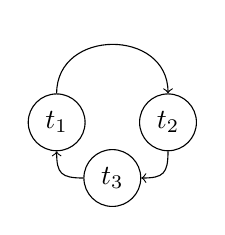
\begin{tikzpicture}[main/.style = {draw, circle}] 
			\node[main] (1) {$t_1$}; 
			\node[main] (3) [below right of=1] {$t_3$}; 
			\node[main] (2) [above right of=3] {$t_2$}; 

			% \draw[->] (1) -- (2);
			\draw[->] (1) to [out=90, in=90, looseness=1.5] (2);
			\draw[->] (2) to [out=270, in=360, looseness=1.5] (3);
			\draw[->] (3) to [out=180, in=270, looseness=1.5] (1);
		\end{tikzpicture} 
	\end{center}

	In the following pages, for metric considerations these terms will be used:

	\begin{itemize}
		\item \texttt{fps}: number of frames per second.
		\item \texttt{for}: time of execution of the elaboration thread.
		\item \texttt{read}: time of execution of the capture thread.
	\end{itemize}

	\subsection{CPU Implementation}
	The CPU implementation is the easier one and the most basic implementation of the algorithm. It consists on a loop between each byte that compose the two frames (the current one and the previous one) and compute the difference, storing it in a new vector.\\

	The C++ implementation is the following:
	\begin{lstlisting}[style=CStyle]
	int total = 3 * ctx.sampleMat->rows * ctx.sampleMat->cols; // no. bytes
	Mat pvs = pready->pframe->clone();
	pready->h_pos = 0;

	for (int i = 0; i < total; i++) {
		int df = pready->pframe->data[i] - previous.data[i];
		if (df < -LR_THRESHOLDS || df > LR_THRESHOLDS) {
			pready->pframe->data[pready->h_pos] = df;
			pready->h_xs[pready->h_pos] = i;
			pready->h_pos++;
		} else {
			pvs.data[i] -= df;
		}
	}

	previous = pvs;
	\end{lstlisting}

	The code here is pretty simple. For each byte, the difference \texttt{df} is computed. If this difference is greater than a fixed threshold \texttt{LR\_THRESHOLDS} it's a good difference so it can be sent. The result of the reconstructed frame at the client side can be seen at Figure \ref{fig:stream_ok}.\\

	\begin{figure}[H]
		\centering
		\includegraphics[width=0.7\linewidth]{images/streaming_ok2.png}
		\caption{\textit{The result of the reconstructed frame}}
		\label{fig:stream_ok}
	\end{figure}
	
	The important point here is that if the difference is too low, it can't be simply discarded, so a kind of negative feedback is needed. This is the purpose of the line of code at line 7, where the value of the byte of the current frame (that at the end of the loop will be the previous for the next iteration) is itself minus the value of the difference. This means that at the next iteration, if that value changes again and its difference increases it will take under consideration as a big difference. Without this, there will be a sum of errors in the reconstructed image, leading in a wrong visualization. The result if the error is not considered can be seen at Figure \ref{fig:stream_error}.
	
	\begin{figure}[H]
		\centering
		\includegraphics[width=0.7\linewidth]{images/streaming_differror.png}
		\caption{\textit{What happens after a certain time if the error is not take under consideration}}
		\label{fig:stream_error}
	\end{figure}

	The performances here are pretty bad. By means of in-code time measurements, the video streaming is stable at 7 fps with an average \texttt{for} time of 140.0 ms and an average \texttt{read} time of 0.0 ms. This means that here the big bottleneck is due to the elaboration part of the software.

	\begin{figure}[H]
		\centering
		\includegraphics[width=0.8\linewidth]{images/chart1.png}
		\caption{\textit{Pixel Difference COmparison}}
	\end{figure}

	\subsection{GPU Implementation}
	The idea is now to port this in the GPU. The GPU can be seen as an accelerator for the CPU, an accelerator that is capable of a high degree of parallelism by executing a lot of simple threads all in parallel in a SIMD way.\\

	In order to port this in CUDA and execute the computation on the GPU, a series of considerations needs to be done. First of all, it's not said that by executing this in GPU there is a direct improvement in performance. This is due to the fact that there is a big bottleneck between the CPU and the GPU and this is the bus that connects them. A GPU in order to do some work on some data needs to have them in its memory (so the GPU can't access directly the CPU's RAM).\\

	The first thing to do, before defining the kernel (the piece of code that is offloaded to the GPU), is to understand how split the 6220800 bytes among the concurrent threads of the GPU. In the Mat object, the frame is rapresented row-major, means that rows are at consecutive address, as shown in Table \ref{tab:row_major}.

	\begin{table}[H]
		\centering
		\begin{tabular}{ |c:c:c| } 
			\hline
			0 & 1 & 2 \\
			\hdashline
			3 & 4 & 5 \\ 
			\hdashline
			6 & 7 & 8 \\ 
			\hline
		\end{tabular}
		\begin{tabular}{ |c|c|c|c|c|c|c|c|c| } 
			\hline
			0 & 0 & 0 & 0 & 0 & 0 & 0 & 0 & 0 \\
			\hdashline
			0x0 & 0x1 & 0x2 & 0x3 & 0x4 & 0x5 & 0x6 & 0x7 & 0x8 \\
			\hline
		\end{tabular}
	\caption{\textit{Row major rapresentation in memory}}
	\label{tab:row_major}
	\end{table}

	Threads can be organized differently according how they access the memory, and in this case there can be two possible cases of memory access per thread:

	\begin{table}[H]
		\parbox{.45\linewidth}{
			\centering
			\begin{tabular}{l|ccc}
				Thread 0 & 0 & 3 & 6\\
				\hline
				Thread 1 & 1 & 4 & 7\\
				\hline
				Thread 2 & 2 & 5 & 8\\
			\end{tabular}
			\caption{Non consecutive access}
		}
		\hfill
		\parbox{.45\linewidth}{
			\centering
			\begin{tabular}{l|ccc}
				Thread 0 & 0 & 1 & 2\\
				\hline
				Thread 1 & 3 & 4 & 5\\
				\hline
				Thread 2 & 6 & 7 & 8\\
			\end{tabular}
			\caption{Consecutive access}
		}
	\end{table}
	
	So the entire array can be divided into <N> chunks where <N> is the number of threads to launch on the GPU. By organizing the kernels in a way they can access the memory in a consecutive access, the kernel will achieve the so called \textit{memory coalesced access}.\\

	How many threads? For a first implementation, and in order to have a modular implementation of the code (so it can be executed on different GPUs with different capabilities), the following code is adopted:

	\begin{lstlisting}[style=CStyle]
	struct cudaDeviceProp prop;
	cudaGetDeviceProperties(&prop, 0); // retrieves device infos

	int total = 3 * ctx.sampleMat->rows * ctx.sampleMat->cols; // no. bytes
	int nMaxThreads = prop.maxThreadsPerBlock;
	int maxAtTime = total / nMaxThreads;
	\end{lstlisting}

	According to this, each thread will work on $N = \textit{maxAtTime}$ consecutive bytes, dividing the memory into \textit{nMaxThreads} chunks, and overlapping is totally avoided.\\

	For what concerns the memory allocation, obviously the CPU address space and the GPU one are two separated things, so a specific allocation on the device side must be done. This can be accomplished thanks to some CUDA's API as follows:

	\begin{lstlisting}[style=CStyle]
	uint8_t *d_current, *d_previous, *d_diff;
	int *d_xs;
	unsigned int *d_pos;

	cudaMalloc((void **)&d_diff, total * sizeof *d_diff);
	cudaMalloc((void **)&d_xs, total * sizeof *d_xs);
	cudaMalloc((void **)&d_current, total * sizeof *d_current);
	cudaMalloc((void **)&d_previous, total * sizeof *d_previous);
	cudaMalloc((void **)&d_pos, sizeof *d_pos);
	\end{lstlisting}


	\subsubsection{Naif version}

	The naif version of the implementation is to port as it is the CPU code into a kernel. From the host side (the CPU) that asks to the device (the GPU) to execute the kernel, there are three kind of operations to be done:

	\begin{enumerate}
		\item copy the frame into the GPU's memory
		\item launch the kernel
		\item copy back the results from the GPU's memory to the HOST memory
	\end{enumerate}

	In the naif implementation, both the previous and current frames are copied into the GPU's memory. At the end of the execution, the results are copied back. This implies 2 transfers HostToDevice (HtoD) for current and previous and 3 transfers DeviceToHost (DtoH) for h\_xs, h\_diff and h\_pos. A memset on the device side is required too to set the initial value of d\_pos to 0.\\

	The host will therefore execute the following operations:

	\begin{lstlisting}[style=CStyle]
	Mat pvs = pready->pframe->clone();
	cudaMemset(d_pos, 0, sizeof *d_pos);

	cudaMemcpy(d_previous, previous.data, total, cudaMemcpyHostToDevice);
	cudaMemcpy(d_current,pready->pframe->data,total,cudaMemcpyHostToDevice);
	kernel<<1,nMaxThreads>>(d_current,d_previous,d_diff,maxAtTime,d_pos,d_xs);
	cudaMemcpy(pready->pframe->data, d_diff, total, cudaMemcpyDeviceToHost);
	cudaMemcpy(pready->h_xs,d_xs,total* sizeof*d_xs,cudaMemcpyDeviceToHost);
	cudaMemcpy(&pready->h_pos, d_pos, sizeof *d_pos, cudaMemcpyDeviceToHost);

	previous = pvs;
	\end{lstlisting}

	It's possible to notice a pretty similar structure of the CPU implementation, where the \textit{for loop} is replaced by the kernel.
	
	// TODO exaplain how start index is computed
	// TODO: explain how to implement the thing about the arrays, the atomicInc, npos and so on
	
	\begin{lstlisting}[style=CStyle]
	__global__ void kernel(
	uint8_t *current, uint8_t *previous, uint8_t *diff, 
	int maxSect, unsigned int *pos, int *xs) {
    int x = threadIdx.x + blockDim.x * blockIdx.x;
    unsigned int npos;
    int df;

    int start = x * maxSect;
    int max = start + maxSect;

    #pragma unroll
    for (int i = start; i < max; i++) {

        df = current[i] - previous[i];
        if (df < -LR_THRESHOLDS || df > LR_THRESHOLDS) {
            npos = atomicInc(pos, 6220801);
            diff[npos] = df;
            xs[npos] = i;
        } else {
            current[i] -= df;
        }

    }

}
	\end{lstlisting}



	TODO:
	\begin{itemize}
		\item Copying both previous and current everytime and no fixed page host allocation
		\item Copying only the current and the previous is a swap pointer, still no fixed page host allocation
		\item Page host allocation
		\item Copy of all d\_diff and d\_xs
		\item Copy first d\_pos then a portion of d\_diff and d\_xs according to d\_pos
		\item Access int-by-int
		\item AtomicInc in global memory and in shared memory, there are differences?
		\item Why 512 kernels is best instead of 1024?
	\end{itemize}

\end{document}